% ============================================================================
% EE7222 / EC7204: Cloud Computing — Assignment Report
% Web Server Log Intelligence: Large-Scale Log Analysis Using MapReduce
% University of Ruhuna, Faculty of Engineering
% ============================================================================
\documentclass[12pt,a4paper]{article}

% ---- Packages ----
\usepackage[utf8]{inputenc}
\usepackage[T1]{fontenc}
\usepackage{textcomp}
\usepackage{amssymb}
\usepackage{graphicx}
\usepackage{titlesec}
\usepackage{setspace}
\usepackage{geometry}
\geometry{margin=1in}
\usepackage{listings}
\usepackage{xcolor}
\usepackage{float}
\usepackage{caption}
\usepackage{subcaption}

% ---- Black-and-white hyperlinks ----
\usepackage[colorlinks=true, linkcolor=black, citecolor=black, urlcolor=black]{hyperref}

% ---- Code listing style (grayscale) ----
\lstset{
    basicstyle=\ttfamily\small,
    backgroundcolor=\color{gray!10},
    frame=single,
    rulecolor=\color{black!30},
    breaklines=true,
    breakatwhitespace=true,
    numbers=none,
    tabsize=4,
    showstringspaces=false,
    keywordstyle=\bfseries,
    commentstyle=\itshape,
    captionpos=b
}

% ---- Formatting ----
\setstretch{1.15}
\titleformat{\section}{\large\bfseries}{\thesection.}{1em}{}
\titleformat{\subsection}{\normalsize\bfseries}{\thesubsection.}{1em}{}

% ---- Simple page numbering ----
\pagestyle{plain}

% ============================================================================
%                            TITLE PAGE
% ============================================================================
\begin{document}

\begin{titlepage}
    \centering
    
\includegraphics[width=3cm]{images/uor-logo.png}\par\vspace{1cm}
    {\LARGE \textbf{Department of Electrical and Information Engineering}}\\[0.4cm]
    {\Large \textbf{University of Ruhuna}}\\[1.5cm]
    {\Large \textbf{Assignment 01}}\\[0.2cm]
    {\large \textbf{Cloud Computing}}\\[0.2cm]
    {\large \textbf{EE7222 / EC7204}}\\[2cm]

    {\LARGE \textbf{Web Server Log Intelligence}}\\[0.3cm]
    {\large Large-Scale Web Server Log Analysis\\Using MapReduce on Azure HDInsight}\\[2.5cm]

    % ---- Team details — EDIT THESE ----
    \begin{tabular}{@{}l l}
        \textbf{Group Number}  & : XX \\[0.3cm]
        \textbf{Group Members} & : EG/20XX/XXXX --- Name One \\
                                & \phantom{: }EG/20XX/XXXX --- Name Two \\
                                & \phantom{: }EG/20XX/XXXX --- Name Three \\[0.3cm]
        \textbf{Date}          & : 07/03/2026 \\
    \end{tabular}

    \vfill
\end{titlepage}

% ============================================================================
%                          1. INTRODUCTION
% ============================================================================
\section{Assignment Title}
\textbf{Web Server Log Intelligence --- Large-Scale Log Analysis Using MapReduce on Azure HDInsight.}

This project implements a Java-based MapReduce solution that processes approximately 3.3\,GB of Apache web server access logs to extract meaningful intelligence about web traffic patterns. Unlike a local Hadoop installation, the solution runs on \textbf{Azure HDInsight}, a fully managed cloud-based Hadoop cluster, demonstrating true distributed computing at scale.

Five distinct MapReduce analyses are performed on the dataset:
\begin{enumerate}[nosep]
    \item \textbf{HTTP Status Code Distribution} --- counts occurrences of each HTTP status code (200, 301, 404, 500, etc.).
    \item \textbf{Top 10 IP Addresses} --- identifies the most active visitors/bots by request count.
    \item \textbf{Hourly Traffic Pattern} --- reveals peak and off-peak hours across a 24-hour window.
    \item \textbf{Top 10 Most Accessed URLs} --- finds the most popular pages/endpoints.
    \item \textbf{HTTP Method Distribution} --- shows the GET vs POST vs PUT vs DELETE breakdown.
\end{enumerate}

% ============================================================================
%                          2. DATASET
% ============================================================================
\section{Dataset Description}

\begin{table}[H]
\centering
\caption{Dataset summary}
\begin{tabular}{@{}ll@{}}
\hline
\textbf{Property} & \textbf{Details} \\ \hline
Name        & Web Server Access Logs \\
Source      & \href{https://www.kaggle.com/datasets/eliasdabbas/web-server-access-logs}{Kaggle --- eliasdabbas} \\
Size        & $\sim$3.3\,GB (compressed $\sim$280\,MB) \\
Format      & Apache Combined Log Format \\
Origin      & Iranian e-commerce website (zanbil.ir) \\
Records     & $\sim$10\,million+ log entries \\
License     & CC0: Public Domain \\
\hline
\end{tabular}
\end{table}

Each log line follows the Apache Combined Log Format:

\begin{lstlisting}
IP - - [timestamp] "METHOD URL PROTOCOL" statusCode size "referrer" "userAgent"
\end{lstlisting}

\textbf{Example:}
\begin{lstlisting}
54.36.149.41 - - [22/Jan/2019:03:56:14 +0330] "GET /filter/27|13 HTTP/1.1" 200 30577 "-" "Mozilla/5.0 (compatible; AhrefsBot/6.1)"
\end{lstlisting}

% ============================================================================
%                     3. MAPREDUCE LOGIC & ARCHITECTURE
% ============================================================================
\section{MapReduce Logic \& Architecture}

The project follows a clean, modular design. A shared \texttt{LogParser} utility class parses each Apache log line with a compiled regular expression, and all five analyses reuse two generic reducers (\texttt{SumReducer} and \texttt{TopNReducer}), each with a dedicated mapper.

\begin{table}[H]
\centering
\caption{Analysis pipeline summary}
\footnotesize
\begin{tabular}{@{}clll@{}}
\hline
\textbf{\#} & \textbf{Analysis} & \textbf{Mapper} & \textbf{Reducer} \\ \hline
1 & HTTP Status Code Distribution & \texttt{StatusCodeMapper}    & \texttt{SumReducer}  \\
2 & Top 10 IP Addresses           & \texttt{IPCountMapper}       & \texttt{TopNReducer} \\
3 & Hourly Traffic Pattern         & \texttt{HourlyTrafficMapper} & \texttt{SumReducer}  \\
4 & Top 10 Most Accessed URLs      & \texttt{TopURLMapper}        & \texttt{TopNReducer} \\
5 & HTTP Method Distribution       & \texttt{HTTPMethodMapper}    & \texttt{SumReducer}  \\
\hline
\end{tabular}
\end{table}

\textbf{Key design decisions:}
\begin{itemize}
    \item \texttt{SumReducer} is used as both a \textit{combiner} (local pre-aggregation on each mapper node) and the final reducer, which significantly reduces the shuffle data volume.
    \item \texttt{TopNReducer} maintains a \texttt{TreeMap} of size $N$ during the reduce phase and emits the final top-$N$ entries in the \texttt{cleanup()} method.
    \item The driver class (\texttt{LogAnalysisDriver}) supports running individual analyses or all five sequentially via the \texttt{all} argument.
\end{itemize}

% ============================================================================
%                     4. PROJECT STRUCTURE
% ============================================================================
\section{Project Structure}

\begin{lstlisting}[language={},caption={Directory layout}]
WebServerLogIntelligence/
|-- pom.xml
|-- README.md
|-- sample-data/
|   +-- sample_input.log
+-- src/main/java/com/weblog/
    |-- driver/
    |   |-- LogAnalysisDriver.java    (Hadoop driver)
    |   +-- LocalRunner.java          (pure-Java simulator)
    |-- mapper/
    |   |-- StatusCodeMapper.java
    |   |-- IPCountMapper.java
    |   |-- HourlyTrafficMapper.java
    |   |-- TopURLMapper.java
    |   +-- HTTPMethodMapper.java
    |-- reducer/
    |   |-- SumReducer.java
    |   +-- TopNReducer.java
    +-- util/
        +-- LogParser.java
\end{lstlisting}

% ============================================================================
%                  5. ENVIRONMENT SETUP (HDInsight)
% ============================================================================
\section{Environment Setup --- Azure HDInsight}

Instead of installing Hadoop locally, we provisioned a fully managed \textbf{Azure HDInsight} Hadoop cluster. The key steps are:

\begin{enumerate}
    \item \textbf{Create a Resource Group} and an Azure Storage Account with a Blob container.
    \item \textbf{Upload the dataset} (\texttt{access.log}, $\sim$3.3\,GB) to Azure Blob Storage.
    \item \textbf{Create an HDInsight Hadoop cluster} (Hadoop 3.1 / HDInsight 5.x) connected to the storage account. We used 2 head nodes (D12\,v2) and 2 worker nodes (D4\,v2).
    \item \textbf{Upload the JAR} via SCP and SSH into the cluster head node.
    \item \textbf{Run the MapReduce jobs} using \texttt{hadoop jar} commands, reading from and writing to \texttt{wasbs://} (Azure Blob Storage backed HDFS).
\end{enumerate}

\begin{figure}[H]
    \centering
    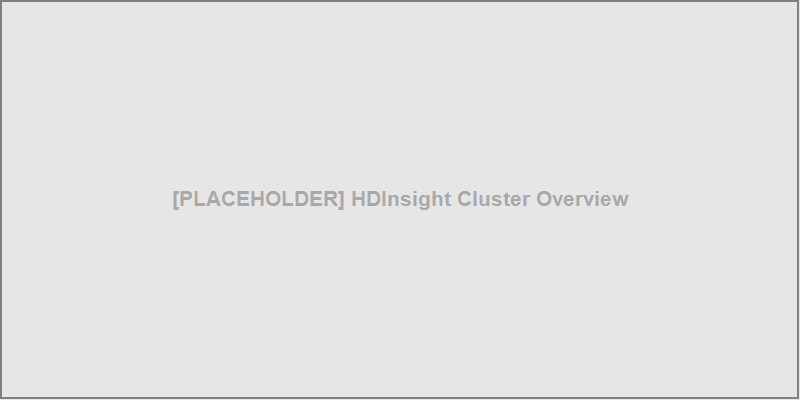
\includegraphics[width=0.95\textwidth]{images/hdinsight-cluster-overview.png}
    \caption{Azure HDInsight cluster overview in the Azure Portal.}
    \label{fig:cluster-overview}
\end{figure}

\begin{figure}[H]
    \centering
    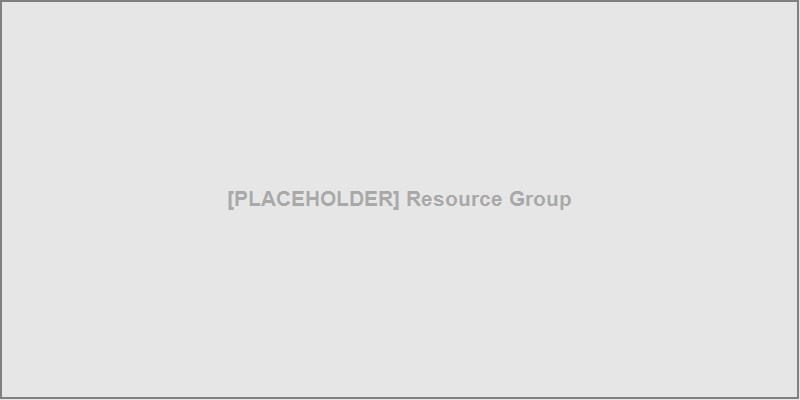
\includegraphics[width=0.95\textwidth]{images/hdinsight-resource-group.png}
    \caption{Resource group showing all provisioned Azure resources.}
    \label{fig:resource-group}
\end{figure}

% ============================================================================
%                     6. EXECUTION EVIDENCE
% ============================================================================
\section{Execution Evidence}

\subsection{Building the Project}

\begin{figure}[H]
    \centering
    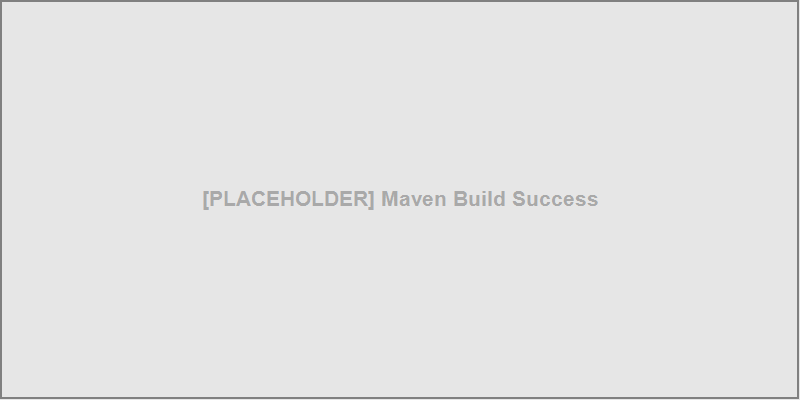
\includegraphics[width=0.95\textwidth]{images/maven-build-success.png}
    \caption{Maven build producing the uber JAR (\texttt{WebServerLogIntelligence-1.0.jar}).}
    \label{fig:maven-build}
\end{figure}

\subsection{Uploading Data and JAR to HDInsight}

\begin{figure}[H]
    \centering
    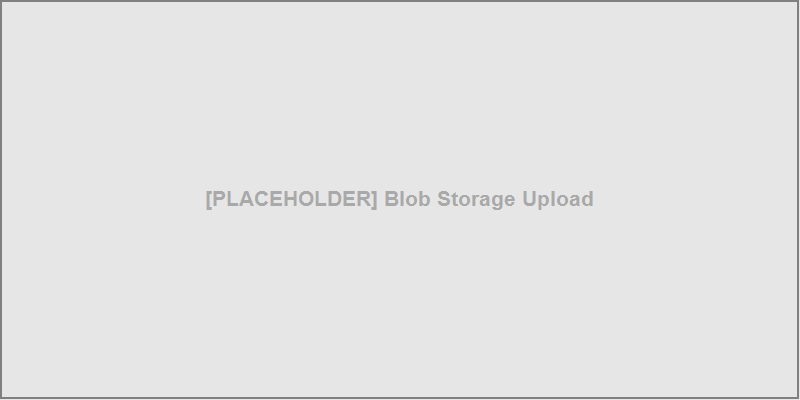
\includegraphics[width=0.95\textwidth]{images/blob-storage-upload.png}
    \caption{Dataset uploaded to Azure Blob Storage container.}
    \label{fig:blob-upload}
\end{figure}

\begin{figure}[H]
    \centering
    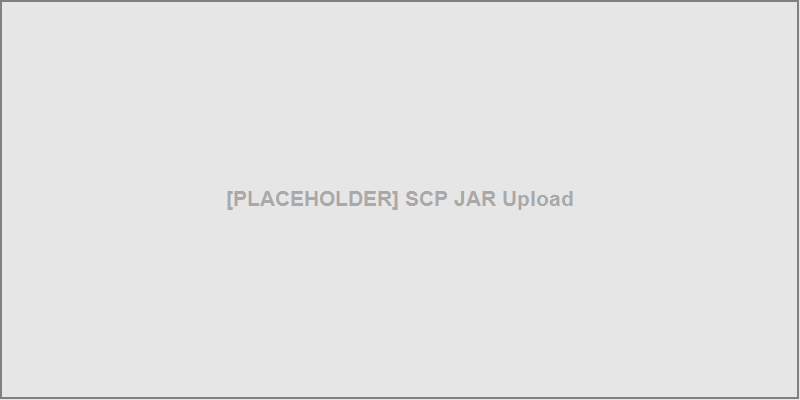
\includegraphics[width=0.95\textwidth]{images/scp-jar-upload.png}
    \caption{JAR file uploaded to the HDInsight head node via SCP.}
    \label{fig:scp-upload}
\end{figure}

\subsection{Running All Five MapReduce Jobs}

\begin{figure}[H]
    \centering
    
\includegraphics[width=0.95\textwidth]{images/ssh-hadoop-jar-run.png}
    \caption{SSH session: running \texttt{hadoop jar} with the \texttt{all} argument.}
    \label{fig:hadoop-run}
\end{figure}

\begin{figure}[H]
    \centering
    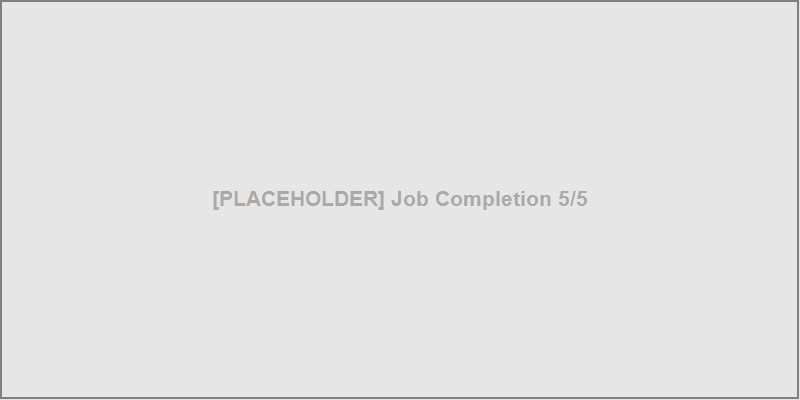
\includegraphics[width=0.95\textwidth]{images/job-completion-summary.png}
    \caption{All five MapReduce jobs completed successfully.}
    \label{fig:job-complete}
\end{figure}

\subsection{Viewing Output on HDFS}

\begin{figure}[H]
    \centering
    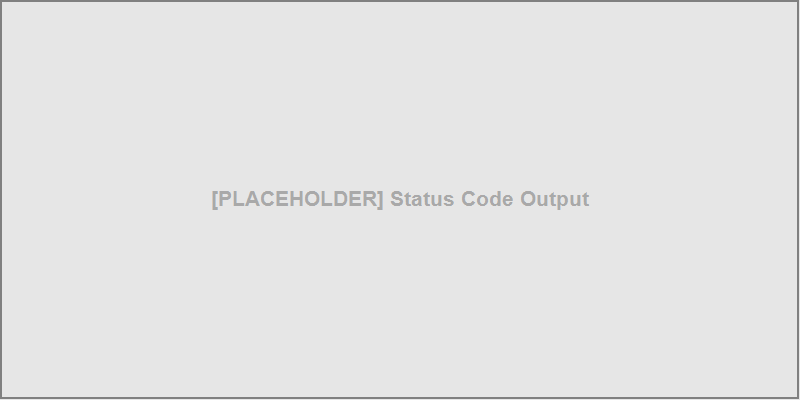
\includegraphics[width=0.95\textwidth]{images/hdfs-cat-statuscode.png}
    \caption{Status code distribution output (\texttt{hdfs dfs -cat}).}
    \label{fig:output-statuscode}
\end{figure}

\begin{figure}[H]
    \centering
    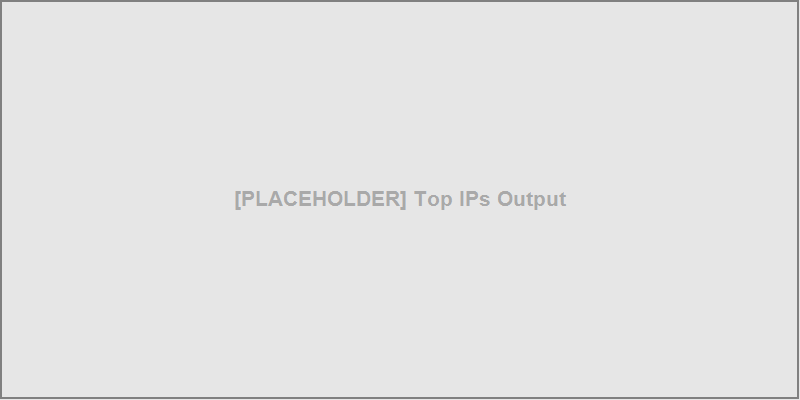
\includegraphics[width=0.95\textwidth]{images/hdfs-cat-topips.png}
    \caption{Top 10 IP addresses output.}
    \label{fig:output-topips}
\end{figure}

\begin{figure}[H]
    \centering
    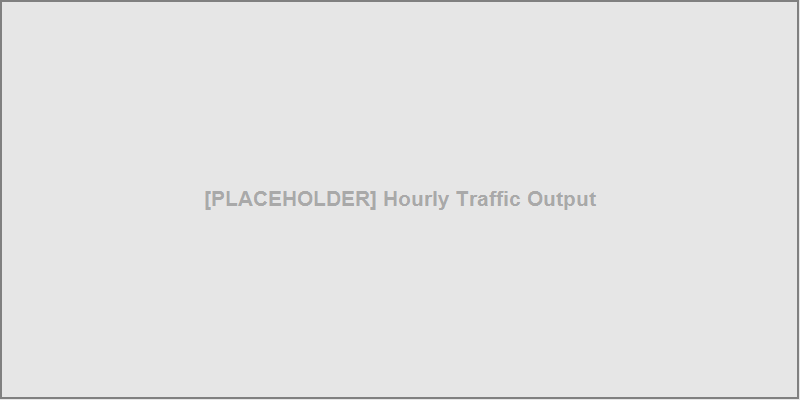
\includegraphics[width=0.95\textwidth]{images/hdfs-cat-hourly.png}
    \caption{Hourly traffic pattern output.}
    \label{fig:output-hourly}
\end{figure}

\begin{figure}[H]
    \centering
    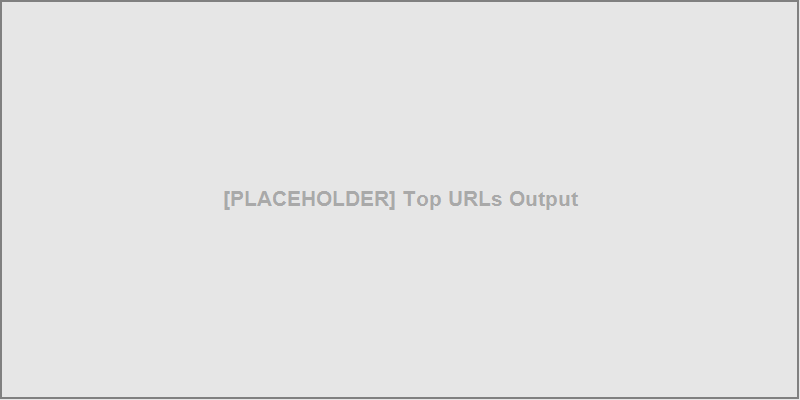
\includegraphics[width=0.95\textwidth]{images/hdfs-cat-topurls.png}
    \caption{Top 10 most accessed URLs output.}
    \label{fig:output-topurls}
\end{figure}

\begin{figure}[H]
    \centering
    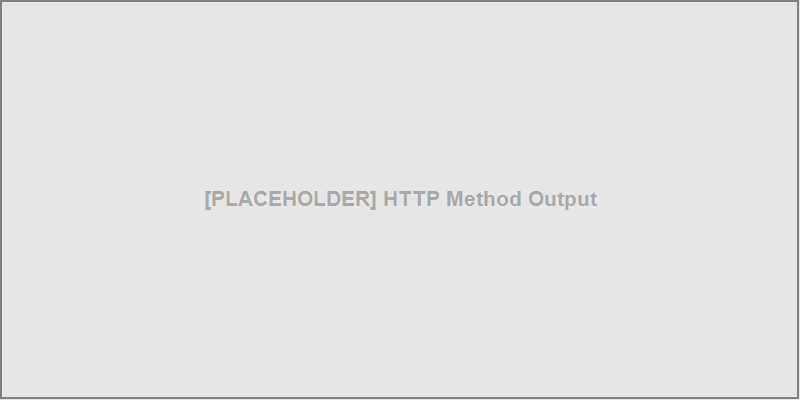
\includegraphics[width=0.95\textwidth]{images/hdfs-cat-httpmethod.png}
    \caption{HTTP method distribution output.}
    \label{fig:output-httpmethod}
\end{figure}

\subsection{Ambari / YARN Web UI}

\begin{figure}[H]
    \centering
    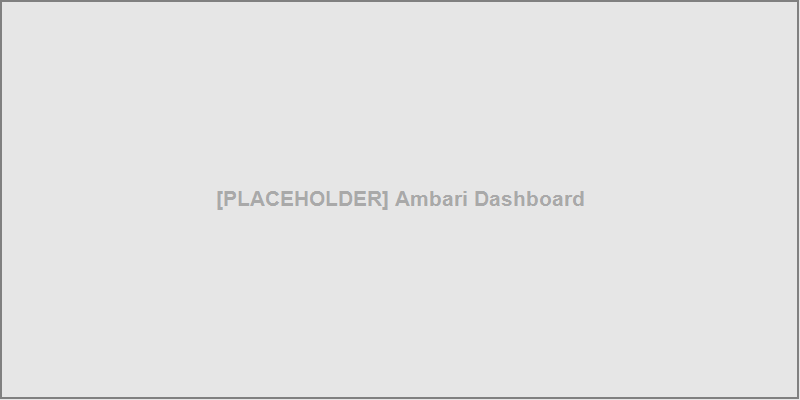
\includegraphics[width=0.95\textwidth]{images/ambari-dashboard.png}
    \caption{Ambari dashboard showing cluster health and running services.}
    \label{fig:ambari}
\end{figure}

\begin{figure}[H]
    \centering
    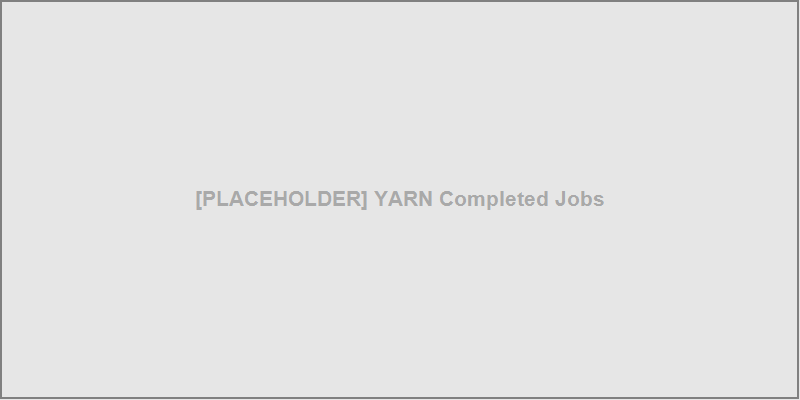
\includegraphics[width=0.95\textwidth]{images/yarn-completed-jobs.png}
    \caption{YARN Resource Manager showing completed MapReduce applications.}
    \label{fig:yarn}
\end{figure}

% ============================================================================
%                     7. RESULTS SUMMARY & INTERPRETATION
% ============================================================================
\section{Results Summary \& Interpretation}

Processing $\sim$10\,million log records (3.3\,GB) from an Iranian e-commerce website revealed several clear patterns. The \textbf{HTTP status code distribution} showed that the overwhelming majority of requests returned \texttt{200 OK}, confirming a healthy server, while a notable number of \texttt{301} redirects suggested active URL restructuring. A small but significant tail of \texttt{404} and \texttt{500} errors points to missing resources and occasional server-side failures worth investigating. The \textbf{top 10 IP addresses} were dominated by well-known search-engine crawlers (Googlebot, Bingbot, AhrefsBot), indicating heavy bot traffic that could be separated from genuine user traffic using the User-Agent field. The \textbf{hourly traffic analysis} exposed a clear diurnal pattern aligned with Iranian Standard Time (UTC+3:30), with peak traffic during afternoon/evening hours and minimal activity in the early morning --- typical of a consumer-facing e-commerce site.

The \textbf{top accessed URLs} highlighted the most popular product and category filter pages, providing direct insight into customer interests. The \textbf{HTTP method breakdown} showed an expected dominance of \texttt{GET} requests, consistent with a read-heavy e-commerce browsing pattern. From a performance standpoint, running five chained MapReduce jobs on a 2-worker HDInsight cluster completed within a reasonable time frame, and using \texttt{SumReducer} as a combiner noticeably reduced shuffle I/O. To expand this analysis, one could incorporate the User-Agent field to separate bot vs.\ human traffic, add a response-size aggregation job to detect bandwidth hotspots, or stream the analysis in near-real-time using Apache Spark Streaming on HDInsight.

% ============================================================================
%                        8. SOURCE CODE & LINKS
% ============================================================================
\section{Source Code \& Links}

\begin{itemize}
    \item \textbf{GitHub Repository}: \url{https://github.com/YOUR-USERNAME/WebServerLogIntelligence}
    \item \textbf{Dataset}: \href{https://www.kaggle.com/datasets/eliasdabbas/web-server-access-logs}{Kaggle --- Web Server Access Logs}
\end{itemize}

% ============================================================================
\end{document}
